\chapter{Implementacija i korisničko sučelje}
		
		
		\section{Korištene tehnologije i alati}
		
			%\textbf{\textit{dio 2. revizije}}
			
			 %\textit{Detaljno navesti sve tehnologije i alate koji su primijenjeni pri izradi dokumentacije i aplikacije. Ukratko ih opisati, te navesti njihovo značenje i mjesto primjene. Za svaki navedeni alat i tehnologiju je potrebno \textbf{navesti internet poveznicu} gdje se mogu preuzeti ili više saznati o njima}.
			 
			 Za ostvarenje komunikacije između članova projektnog tima korištena je aplikacija WhatsApp\footnote{\url{https://www.whatsapp.com/}}. Za održavanje sastanaka unutar tima korištena je platforma MS Teams\footnote{\url{https://www.microsoft.com/microsoft-teams/}}. Komunikacija s demonstratorom i asistentom ostvarena je također s pomoću platforme MS Teams. Praćenje napretka i raspodjela zadataka u timu ostvarena je pomoću alata Jira\footnote{\url{https://www.atlassian.com/software/jira}}. Jira pomoću tzv. issue nudi mogućnost podijele izrade u manje zadatke koji se zatim mogu pridijeliti nekom od članova tima. Svaki od člana tima zatim može za svaki zadatak prikazati u kojoj je fazi izrade što ostalim članovima nudi mogućnost uvida u to na čemu drugi članovi tima trenutno rade. Upravljanje izvornim kodom i dokumentacijom ostvareno je s pomoću alata Git\footnote{\url{https://git-scm.com/}}. Udaljeni repozitorij pohranjen je na platformi GitHub\footnote{\url{https://github.com/}}. Za izradu dokumentacije projekta korišten je LaTeX\footnote{\url{https://www.latex-project.org/}}. UML dijagram obrazaca uporabe, sekvencijski dijagram, prva revizija dijagrama razreda, dijagram aktivnosti, dijagram stanja, dijagram komponenti i dijagram razmještaja napravljeni su s pomoću alata Astah UML\footnote{\url{https://astah.net/products/astah-uml/}}. Implementacijski dijagram razreda napravljen je s pomoću alata IntelliJ IDEA\footnote{\url{https://www.jetbrains.com/idea/}}. Model baze podataka izgrađen je alatom ERDPlus\footnote{\url{https://erdplus.com/}}. Dizajn dijelova sustava ostvaren je alatom Figma\footnote{\url{https://www.figma.com/}} Za izradu backend dijela aplikacije korišten je radni okvir Java\footnote{\url{https://www.java.com/en/}} Spring\footnote{\url{https://spring.io/}}, a za razvoj na backendu korišteno je razvojno okruženje IntelliJ IDEA. Za izradu frontend dijela aplikacije korištena je knjižnica React\footnote{\url{https://react.dev/}} uz programski jezik TypeScript\footnote{\url{https://www.typescriptlang.org/}}. Za ispitivanje sustava korišteni su JUnit\footnote{\url{https://junit.org/}} i Selenium\footnote{\url{https://www.selenium.dev/}}. Za puštanje aplikacije u pogon korištena je platforma Render\footnote{\url{https://render.com/}}.
			
			
			\eject 
		
	
		\section{Ispitivanje programskog rješenja}

			\subsection{Ispitivanje komponenti}
			
			\subsubsection{Testiranje Gettera i Settera}
			
			TestGettersAndSetters služi za provjeru ispravnosti gettera i settera za klasu \texttt{Account}. U ovom testu se inicijalizira objekt \texttt{Account} s određenim podacima (email, ime, prezime, lozinka, i uloga), a zatim se koriste getteri za dohvaćanje tih podataka i setteri za postavljanje novih vrijednosti. Nakon postavljanja novih vrijednosti, ponovno se koriste getteri za provjeru je li objekt uspješno promijenjen prema očekivanjima.
			
			\begin{lstlisting}[language=Java]
@Test
public void testGettersAndSetters() {
	Account account = new Account("test@example.com", "John", 
				"Doe", "password", Roles.USER);
	
	Assertions.assertEquals("test@example.com", 
				account.getEmail());
	Assertions.assertEquals("John", account.getFirstName());
	Assertions.assertEquals("Doe", account.getLastName());
	Assertions.assertEquals("password", account.getPassword());
	Assertions.assertEquals(Roles.USER, account.getRole());
	
	account.setEmail("newemail@example.com");
	account.setFirstName("Jane");
	account.setLastName("Smith");
	account.setPassword("newpassword");
	account.setRole(Roles.ADMIN);
	
	Assertions.assertEquals("newemail@example.com", 
				account.getEmail());
	Assertions.assertEquals("Jane", account.getFirstName());
	Assertions.assertEquals("Smith", account.getLastName());
	Assertions.assertEquals("newpassword", account.getPassword());
	Assertions.assertEquals(Roles.ADMIN, account.getRole());
}
			\end{lstlisting}
			
			\subsubsection{Testiranje Token Verzije}
			
			TestTokenVersion provjerava funkcionalnost metoda za rad s token verzijom \\(\texttt{getTokenVersion()}, \texttt{incrementTokenVersion()}, \texttt{setTokenVersion()}) za klasu \texttt{Account}. Prvo se inicijalizira objekt \texttt{Account}, a zatim se provjerava da li je početna vrijednost token verzije jednaka 0. Nakon toga, koristi se metoda \texttt{incrementTokenVersion()} za povećanje verzije za 1 i provjerava se da li je nova vrijednost 1. Također se koristi metoda \texttt{setTokenVersion()} za postavljanje verzije na 5 i provjerava se je li postavljena vrijednost ispravna.
			
			\begin{lstlisting}[language=Java]
@Test
public void testTokenVersion() {
	Account account = new Account("test@example.com", "John", 
				"Doe", "password", Roles.USER);
	
	Assertions.assertEquals(0L, account.getTokenVersion());
	
	account.incrementTokenVersion();
	Assertions.assertEquals(1L, account.getTokenVersion());
	
	account.setTokenVersion(5L);
	Assertions.assertEquals(5L, account.getTokenVersion());
}
			\end{lstlisting}
			
			\subsubsection{Testiranje Metode \texttt{toString()}}
			
			ToString test provjerava da li metoda \texttt{toString()} klase \texttt{Account} vraća očekivani format teksta. Prvo se inicijalizira objekt \texttt{Account} s određenim podacima, a zatim se koristi metoda \texttt{toString()} za dobivanje string reprezentacije objekta. Očekivana string reprezentacija se uspoređuje s unaprijed definiranom očekivanom vrijednošću.
			
			\begin{lstlisting}[language=Java]
@Test
public void testToString() {
	Account account = new Account("test@example.com", "John", 
			"Doe", "password", Roles.USER);
	
	String expectedToString = "Account{" +
		"id=null" +
		", email='test@example.com'" +
		", firstName='John'" +
		", lastName='Doe'" +
		", password='password'" +
		", role=USER" +
		", tokenVersion=0" +
		'}';
	
	Assertions.assertEquals(expectedToString, account.toString());
}
			\end{lstlisting}
			
			\subsubsection{Testiranje Metode \texttt{testLoadUserByUsername\char`_ThrowsException()}}
			
			Koristi se Assertions.assertThrows iz JUnit frameworka kako bi se provjerilo da će poziv loadUserByUsername(email) metode iz accountUserDetailsService doista izazvati iznimku tipa UsernameNotFoundException. Očekuje se da metoda loadUserByUsername baci iznimku kada korisnik s navedenim emailom ne postoji u sustavu.
			
			\begin{lstlisting}[language=Java]
@Test
public void testLoadUserByUsername_ThrowsException() {
	String email = "test@example.com";
	
	when(accountService.findByEmail(email))
		.thenReturn(Optional.empty());
	
	Assertions.assertThrows(
		UsernameNotFoundException.class, () -> {
			accountUserDetailsService
			.loadUserByUsername(email);
	});
}
			\end{lstlisting}
			
			\subsubsection{Testiranje Metode \texttt{testGetAllDicts\char`_EmptyList()}}	
			
			\begin{itemize}
				\item \textbf{Arrange}: Postavlja se ponašanje mock objekta \texttt{dictionaryService} kako bi simulirali situaciju kada nema rječnika. Očekujemo da će \texttt{dictionaryService.getAllDicts()} vratiti praznu listu koristeći \texttt{when} metodu.
				
				\item \textbf{Act}: Poziva se \texttt{GET()} metoda iz \texttt{dictionaryController} kako bi se dobio odgovor.
				
				\item \textbf{Assert}: Provjerava se da li je odgovor tipa \texttt{HttpStatus.NOT\_FOUND} (404), što označava da nema dostupnih rječnika. Također se provjerava da li je tijelo odgovora prazna lista (\texttt{Collections.emptyList()}).
				
				\item \textbf{Verify}: Koristi se \texttt{verify} kako bi se provjerilo da je \texttt{dictionaryService.getAllDicts()} pozvana točno jednom i da nije bilo više interakcija s tim servisom \\(\texttt{verifyNoMoreInteractions(dictionaryService)}).
			\end{itemize}
			
			\begin{lstlisting}[language=Java]
				
@Test
public void testGetAllDicts_EmptyList() {
	// Arrange
	when(dictionaryService.getAllDicts())
		.thenReturn(Collections.emptyList());
	
	// Act
	ResponseEntity<List<Dictionary>> response = 
		dictionaryController.GET();
	
	// Assert
	Assertions.assertEquals(HttpStatus.NOT_FOUND, 
		response.getStatusCode());
	Assertions.assertEquals(Collections.emptyList(), 
		response.getBody());
	
	verify(dictionaryService, times(1)).getAllDicts();
	verifyNoMoreInteractions(dictionaryService);
}
				
			\end{lstlisting}
			
			\subsubsection{Testiranje Metode \texttt{testGetAllDicts\char`_NonEmptyList()}}	
			
			\begin{itemize}
				\item \textbf{Arrange}: Postavlja se ponašanje mock objekta \texttt{dictionaryService} kako bi simulirali situaciju kada lista rječnika sadrži nekoliko rječnika. Očekujemo da će \texttt{dictionaryService.getAllDicts()} vratiti listu rječnika koristeći \texttt{when} metodu.
				
				\item \textbf{Act}: Poziva se \texttt{GET()} metoda iz \texttt{dictionaryController} kako bi se dobio odgovor.
				
				\item \textbf{Assert}: Provjerava se da li je odgovor tipa \texttt{HttpStatus.OK} (200), što označava uspješan zahtjev, te da li tijelo odgovora sadrži listu rječnika koja je vraćena iz \texttt{dictionaryService}.
				
				\item \textbf{Verify}: Koristi se \texttt{verify} kako bi se provjerilo da je \texttt{dictionaryService.getAllDicts()} pozvana točno jednom i da nije bilo više interakcija s tim servisom (\texttt{verifyNoMoreInteractions(dictionaryService)}).
			\end{itemize}
			
			\begin{lstlisting}[language=Java]
				
@Test
public void testGetAllDicts_NonEmptyList() {
	// Arrange
	List<Dictionary> dictionaries = List
		.of(new Dictionary(), new Dictionary());
	when(dictionaryService.getAllDicts())
		.thenReturn(dictionaries);
	
	// Act
	ResponseEntity<List<Dictionary>> response = 
		dictionaryController.GET();
	
	// Assert
	Assertions.assertEquals(HttpStatus.OK, 
		response.getStatusCode());
	Assertions.assertEquals(dictionaries, response.getBody());
	
	verify(dictionaryService, times(1)).getAllDicts();
	verifyNoMoreInteractions(dictionaryService);
}
				
			\end{lstlisting}
			
			\subsection{Ispitivanje sustava}
			
			Ispitivanje sustava provodi se korištenjem Selenium WebDrivera i programskog jezika Java. U nastavku su opisana četiri testa, te su priloženi programski kodovi.
			
			\subsubsection{Testiranje prijave}

			U ovom testu koristi se Selenium WebDriver za otvaranje web preglednika (Chrome) i prijavu na web stranicu. Nakon prijave, provjerava se trenutna URL adresa. Ako URL sadrži "/home", to znači da je prijava uspješna i ispisuje se poruka "Login successful!". Inače, ispisuje se poruka "Login failed!".

			\begin{lstlisting}
System.setProperty("webdriver.chrome.driver", 
	"C:\\Users\\Korisnik\\Desktop\\chromedriver.exe");
WebDriver driver = new ChromeDriver();
driver.get("http://localhost:3000/login");

driver.manage().window().maximize();
driver.findElement(By.name("email")).sendKeys("admin");
driver.findElement(By.name("password")).sendKeys("password");

WebElement button = driver.findElement(By.className("accentBtn"));
button.click();

driver.getCurrentUrl().then((url) -> {
	if (url.contains("/home")) {
		System.out.println("Login successful!");
	} else {
		System.err.println("Login failed!");
	}
	driver.quit();        
});	

			\end{lstlisting}
			
			\subsubsection{Testiranje registracije}

			U sljedećem isječku koda prikazano je testiranje registracije na web stranici:
			
			\begin{lstlisting}
driver.get("http://localhost:3000/login");
// Perform additional test steps
driver.manage().window().maximize();
WebElement anchorTag = driver.findElement(
	By.className("login_createAccountLink__FV3W+"));
anchorTag.click();
WebElement firstNameField = driver.findElement(
	By.name("firstName"));
WebElement lastNameField = driver.findElement
	(By.name("lastName"));
WebElement emailField = driver.findElement(By.name("email"));

firstNameField.sendKeys("John");
lastNameField.sendKeys("Doe");
emailField.sendKeys("johndoe@fer.com");

WebElement registerButton = driver.findElement(
	By.className("accentBtn"));
registerButton.click();
driver.getCurrentUrl().then((url) -> {
	if (url.contains("/changepass")) {
		System.out.println("registration successful!");
	} else {
		System.err.println("Registration failed!");
	}
	driver.quit();        
});
			\end{lstlisting}

			\subsubsection{Testiranje klika na element}

			U ovom testu otvara se web stranica na URL adresi "http://localhost:3000/home" i izvode se određene akcije na web stranici (u ovom slučaju, klik na određeni element). Nakon izvršenja akcija, provjerava se trenutna URL adresa. Ako URL sadrži "/home/en", to znači da su akcije uspješno izvršene i ispisuje se poruka "Successful!". Inače, ispisuje se poruka "Failed!".

			\begin{lstlisting}
driver.get("http://localhost:3000/home");

driver.manage().window().maximize();
WebElement element = driver.findElement(
	By.xpath("//div[@class='card_card__611WY']"));
element.click();

driver.getCurrentUrl().then((url) -> {
	if (url.contains("/home/en")) {
		System.out.println("Successful!");
	} else {
		System.err.println("Failed!");
	}
	driver.quit();
});
			\end{lstlisting}

			\subsubsection{Testiranje ponovne prijave}

			U sljedećem isječku koda prikazano je testiranje ponovne prijave na web stranicu koje bi zbog ne unosa passworda trebalo završiti neuspješno.

			\begin{lstlisting}
driver.get("http://localhost:3000/login");

driver.manage().window().maximize();
driver.findElement(By.name("email")).sendKeys("admin");

WebElement button = driver.findElement(By.className("accentBtn"));
button.click();

driver.getCurrentUrl().then((url) -> {
	if (url.contains("/home")) {
		System.out.println("Login successful!");
	} else {
		System.err.println("Login failed!");
	}
	driver.quit();        
});
			\end{lstlisting}


		
		
		\section{Dijagram razmještaja}
			
			%\textbf{\textit{dio 2. revizije}}
			
			 %\textit{Potrebno je umetnuti \textbf{specifikacijski} dijagram razmještaja i opisati ga. Moguće je umjesto specifikacijskog dijagrama razmještaja umetnuti dijagram razmještaja instanci, pod uvjetom da taj dijagram bolje opisuje neki važniji dio sustava.}
			 
			 \begin{figure}[H]
			 	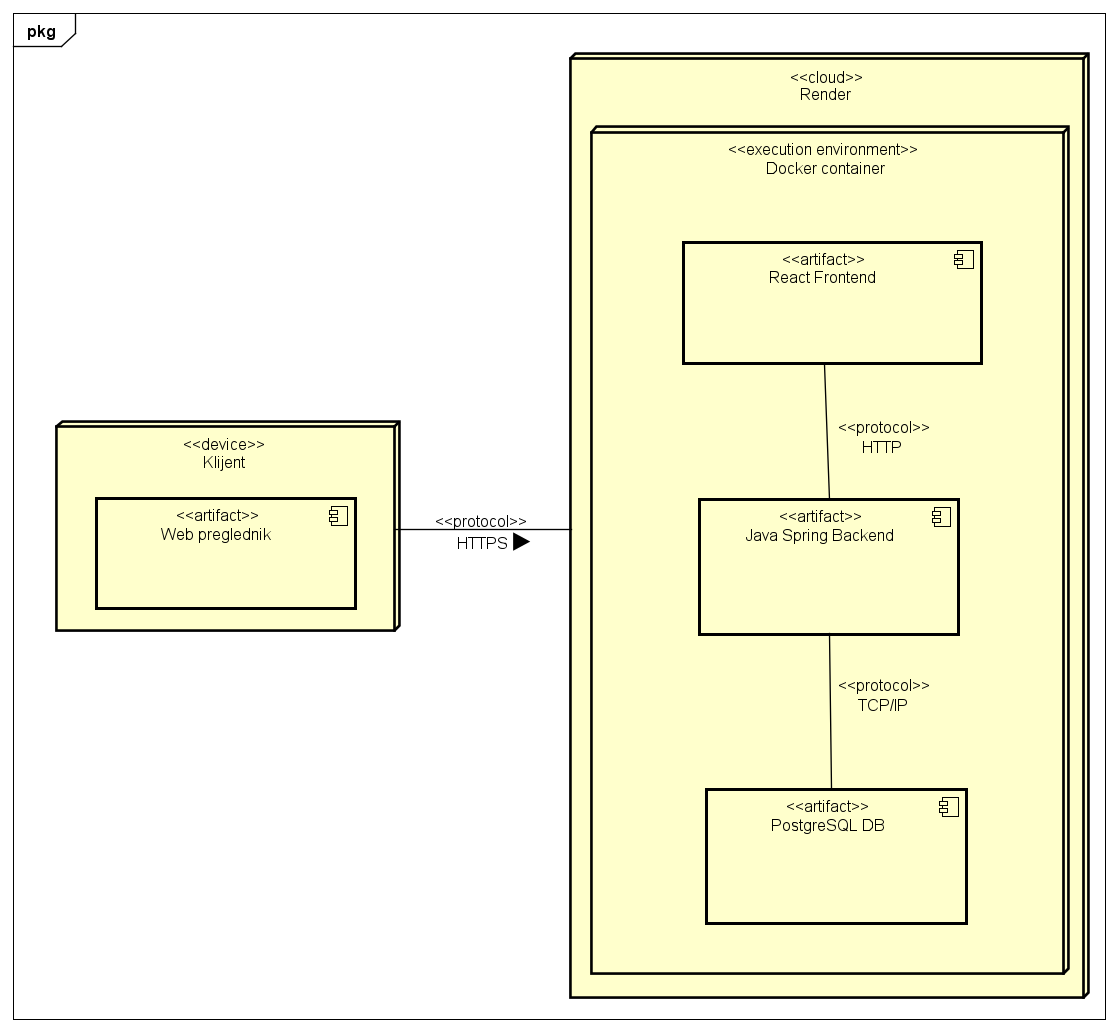
\includegraphics[width=\textwidth]{slike/DeploymentDiagram.PNG}
			 	\caption{Dijagram razmještaja}
			 	\label{fig:deploymentDiagram}
			 \end{figure}
			 
			 \newpage
			 
			 Slika 5.1 prikazuje dijagram razmještaja. Dijagram razmještaja prikazuje raspodjelu programskih komponenti kao što su izvršne datoteke i virtualna izvršna okruženja. Dijagram se sastoji od dvaju glavnih čvorova nazvanih Klijent i Render. Čvor Klijent predstavlja uređaj kojim klijent, odnosno korisnik pokušava pristupiti sustavu. Čvor se sastoji od jednog artefakta, Web preglednika. Web preglednik je izvršna datoteka kojom korisnik šalje sve zahtjeve u sustav i prima odgovore iz sustava. Drugi čvor na dijagramu je Render. Render je poslužiteljsko računalo/a koja su smještena u oblaku. Cijela aplikacija je smještena unutar kontejnera Docker u oblaku Render. Kontejner Docker je virtualno izvršno okruženje. Pripadni čvor Docker container je ugniježđen unutar čvora Render. Frontend dio aplikacije implementiran je kao React aplikacija, backend dio implementiran je koristeći Java Spring radni okvir, a baza podataka koja služi da pohranu svih potrebnih podataka implementirana je kao PostgreSQL. Komunikacija između korisnika, odnosno web preglednika i aplikacije odvija se preko HTTPS protokola, protokola na aplikacijskom sloju. Svaki od artefakata koji zajedno čine aplikaciju, međusobno komuniciraju. Komunikacija između frontend i backend dijela aplikacije izvodi se preko HTTP protokola, dok se komunikacija između Java Spring backenda i baze podataka izvodi s pomoću protokola nižih slojeva, točnije TCP/IP protokolima.
			
			\eject 
		
		\section{Upute za puštanje u pogon}
		
%			\textbf{\textit{dio 2. revizije}}\\
		
%			 \textit{U ovom poglavlju potrebno je dati upute za puštanje u pogon (engl. deployment) ostvarene aplikacije. Na primjer, za web aplikacije, opisati postupak kojim se od izvornog kôda dolazi do potpuno postavljene baze podataka i poslužitelja koji odgovara na upite korisnika. Za mobilnu aplikaciju, postupak kojim se aplikacija izgradi, te postavi na neku od trgovina. Za stolnu (engl. desktop) aplikaciju, postupak kojim se aplikacija instalira na računalo. Ukoliko mobilne i stolne aplikacije komuniciraju s poslužiteljem i/ili bazom podataka, opisati i postupak njihovog postavljanja. Pri izradi uputa preporučuje se \textbf{naglasiti korake instalacije uporabom natuknica} te koristiti što je više moguće \textbf{slike ekrana} (engl. screenshots) kako bi upute bile jasne i jednostavne za slijediti.}
			
			
%			 \textit{Dovršenu aplikaciju potrebno je pokrenuti na javno dostupnom poslužitelju. Studentima se preporuča korištenje neke od sljedećih besplatnih usluga: \href{https://aws.amazon.com/}{Amazon AWS}, \href{https://azure.microsoft.com/en-us/}{Microsoft Azure} ili \href{https://www.heroku.com/}{Heroku}. Mobilne aplikacije trebaju biti objavljene na F-Droid, Google Play ili Amazon App trgovini.}

			\hspace*{6mm}U ovom poglavlju dane su upute za puštanje aplikacije u pogon na usluzi Render. Slika 5.2 prikazuje početnu stranicu na kojoj će se izvršavati puštanje u pogon. Za puštanje u pogon potrebno je pripremiti Docker kontejner koji će uspješno izgraditi aplikaciju. Na prikazanoj slici već postoji web servis i baza podataka, no u nastavku su dane upute za njihovo stvaranje. 

			\begin{figure}[H]
				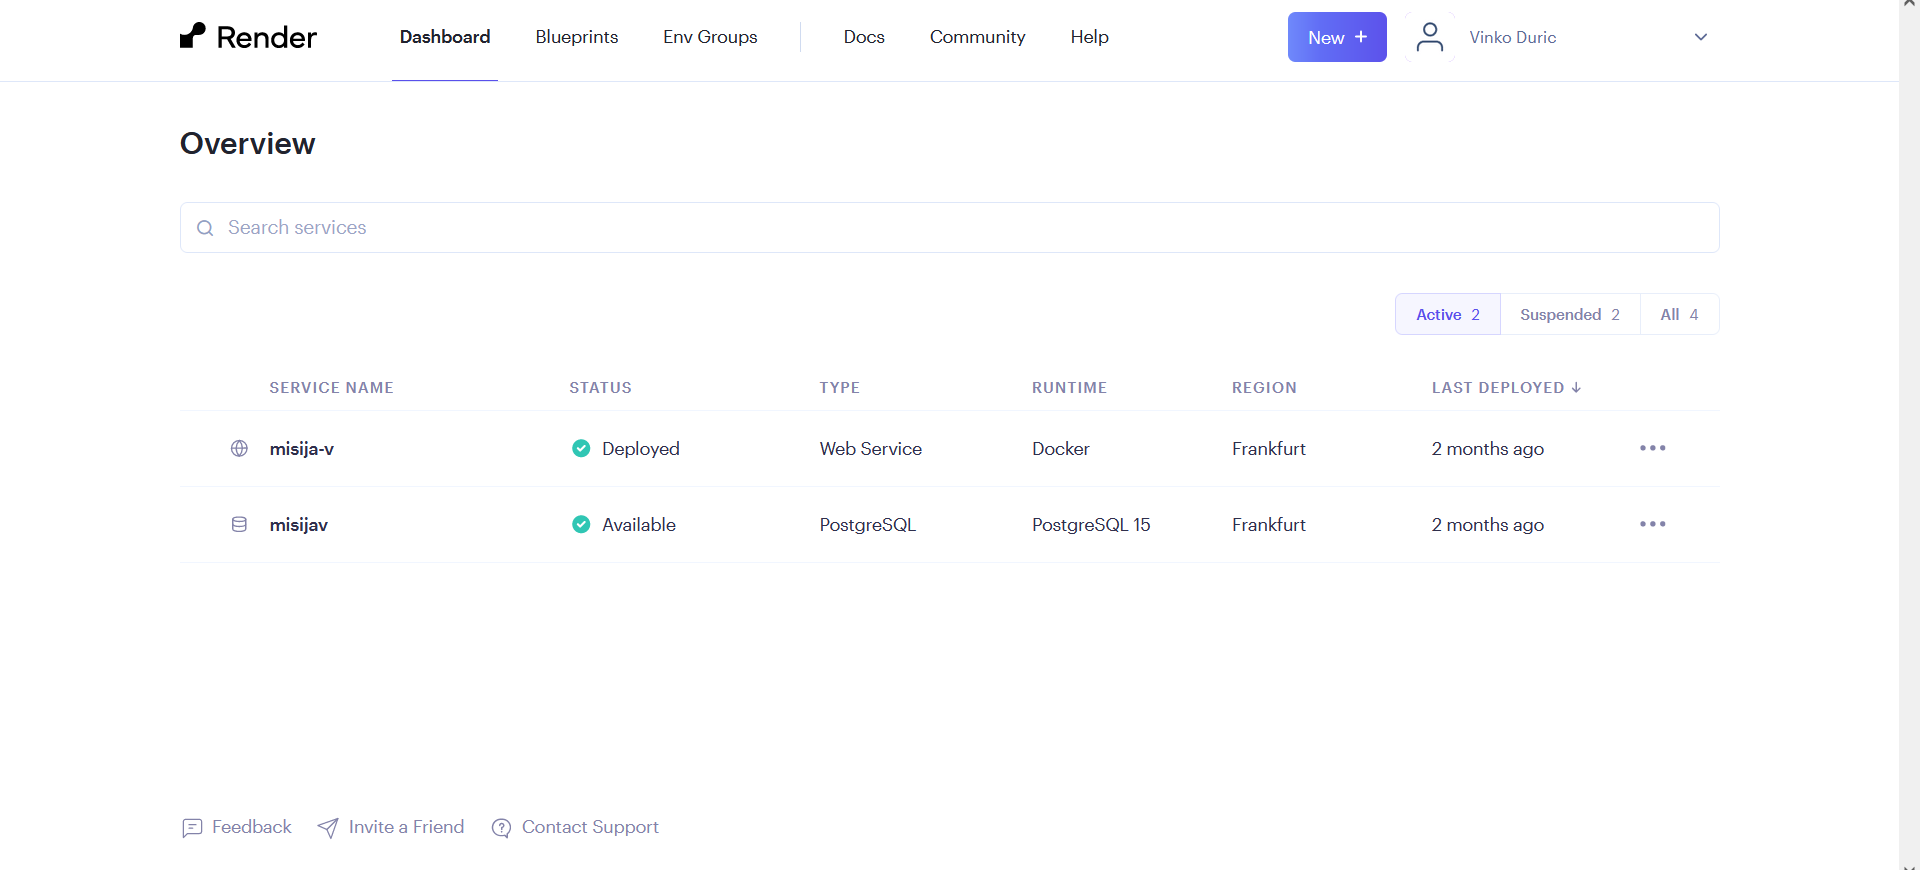
\includegraphics[width=\textwidth]{slike/deploy1.PNG}
				\caption{Render - početna stranica}
				\label{fig:deployment1}
			\end{figure}
			
			Slika 5.3 prikazuje izbornik koji otvaramo klikom na gumb "New". Za početak je potrebno napraviti bazu podataka pa stoga odabiremo opciju "PostgreSQL".
			
			\begin{figure}[H]
				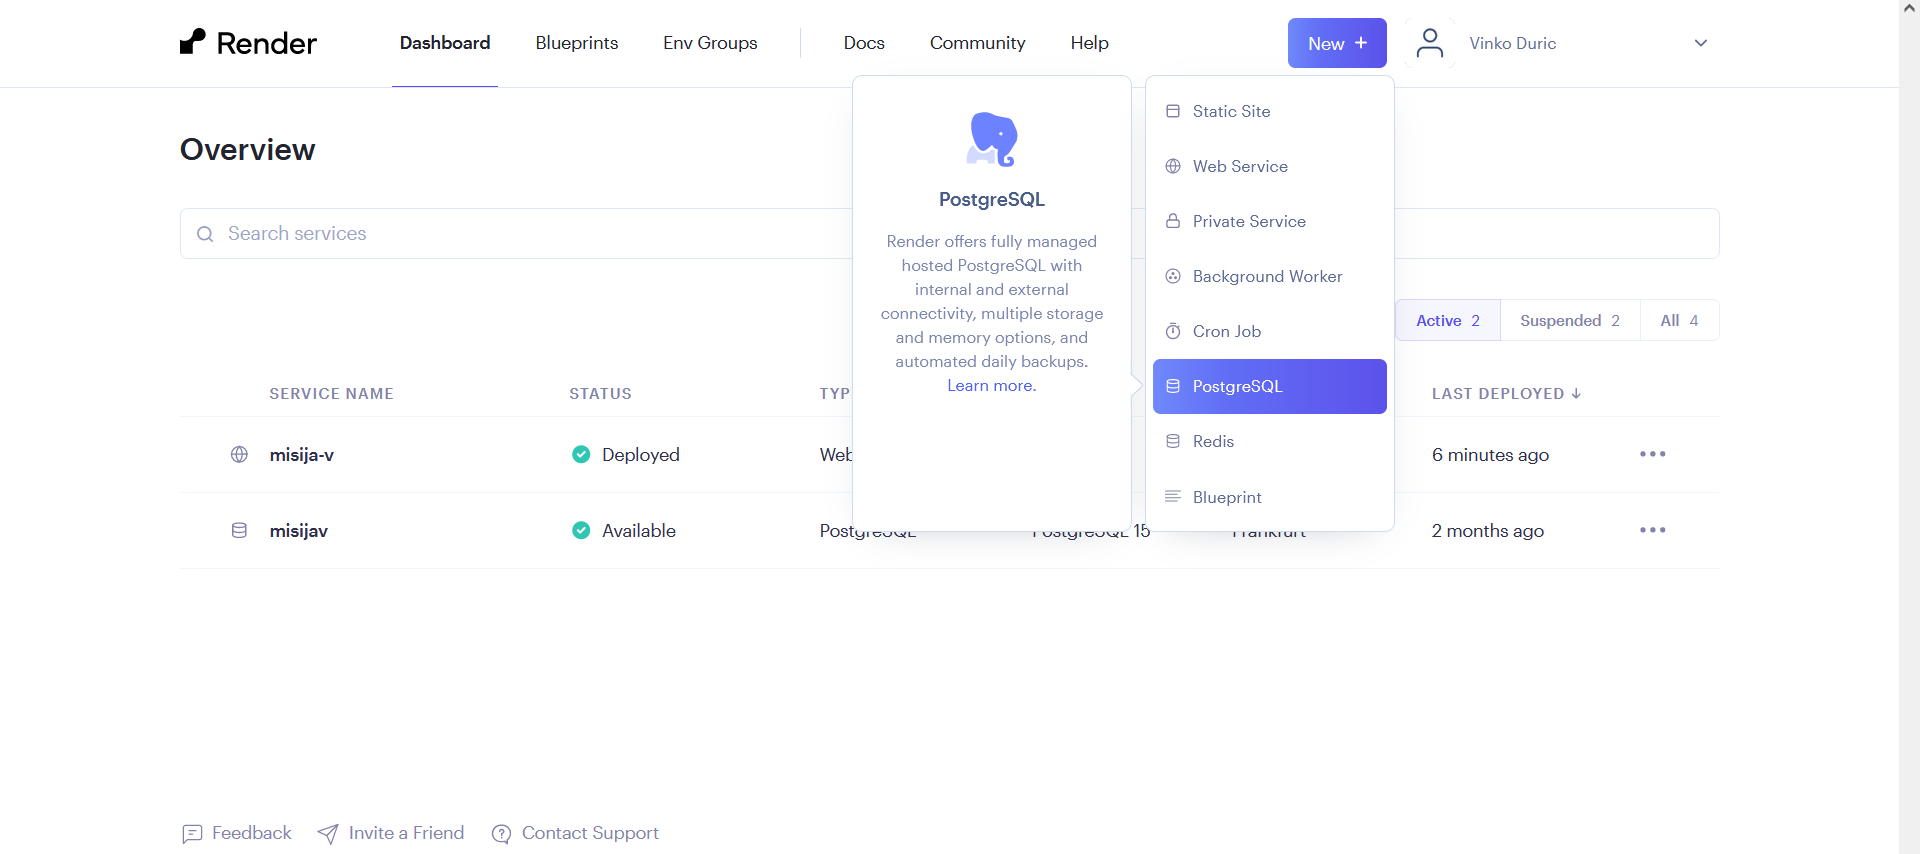
\includegraphics[width=\textwidth]{slike/deploy2.PNG}
				\caption{Render - stvaranje novih servisa}
				\label{fig:deployment2}
			\end{figure}
			
			Na slici 5.4 prikazana je stranica u kojoj je potrebno ispuniti sve potrebne podatke o bazi podataka za njezino uspješno kreiranje.
			
			\begin{figure}[H]
				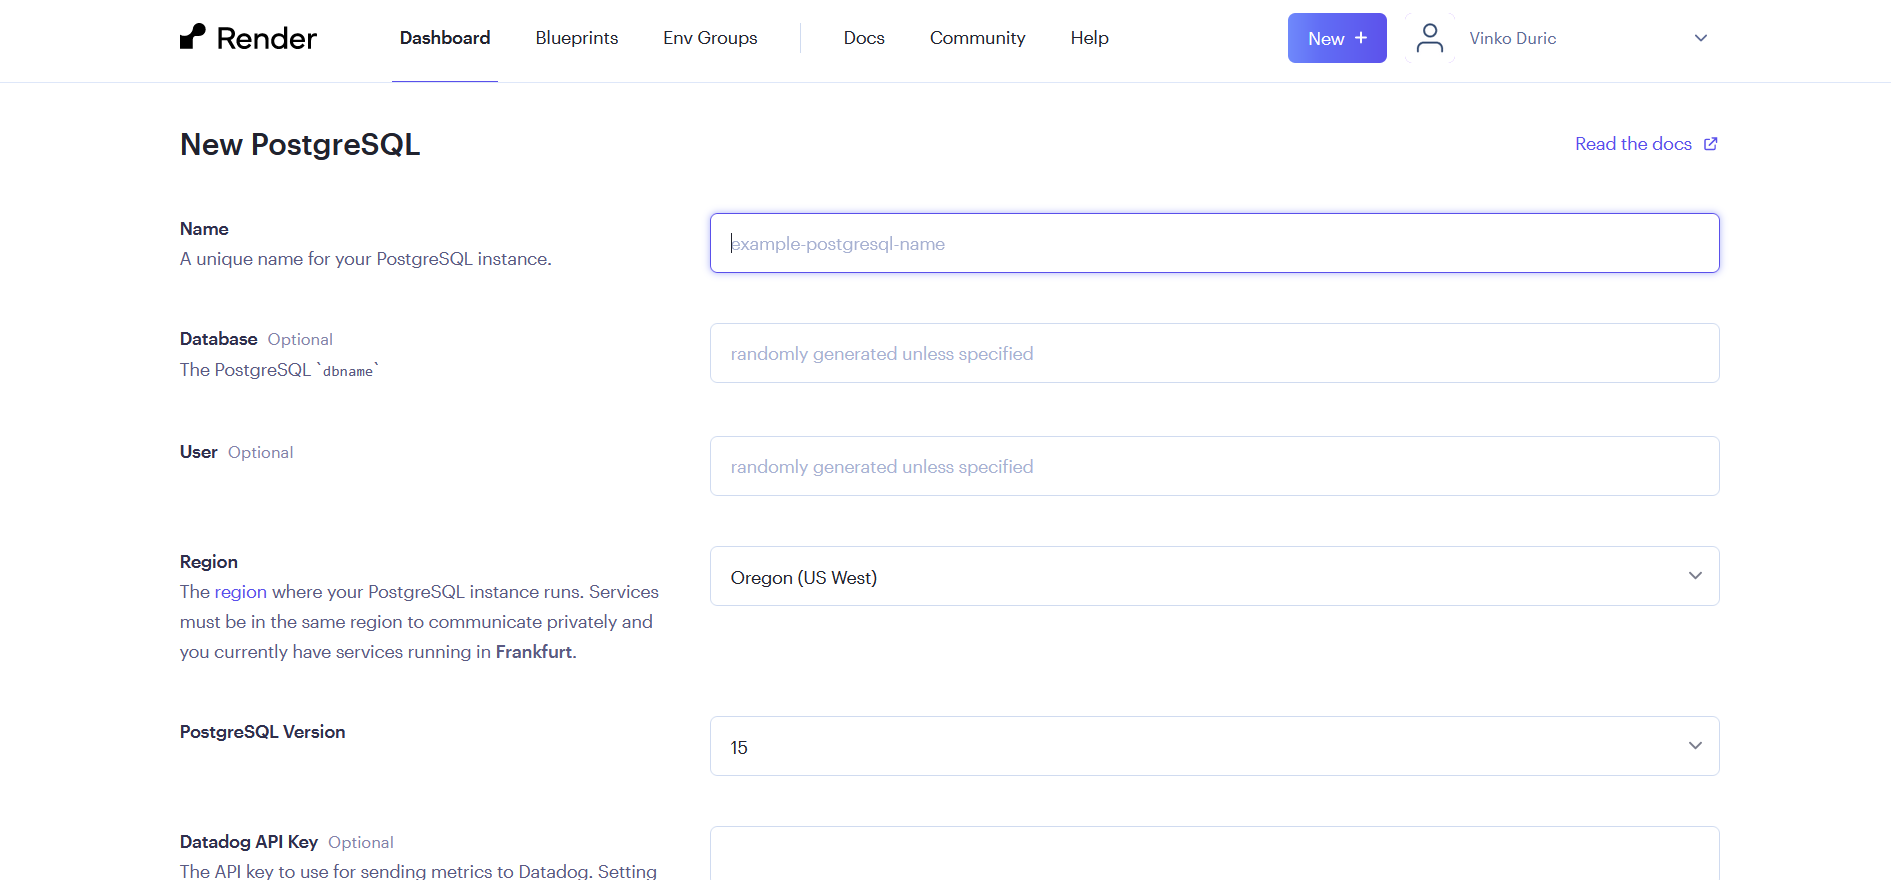
\includegraphics[width=\textwidth]{slike/deploy3.PNG}
				\caption{Render - stvaranje nove baze podataka}
				\label{fig:deployment3}
			\end{figure}
			
			Nakon ispunjavanja svih potrebnih podataka, kreirana je baza podataka. Kada s početne stranice prikazane na slici 5.1 odaberemo našu bazu podataka (koja će se tamo pojaviti samim kreiranjem) možemo vidjeti sve potrebne podatke, a neki podaci koji će nam biti važni u nastavku puštanja u pogon prikazani su na slici 5.5.
			
			\begin{figure}[H]
				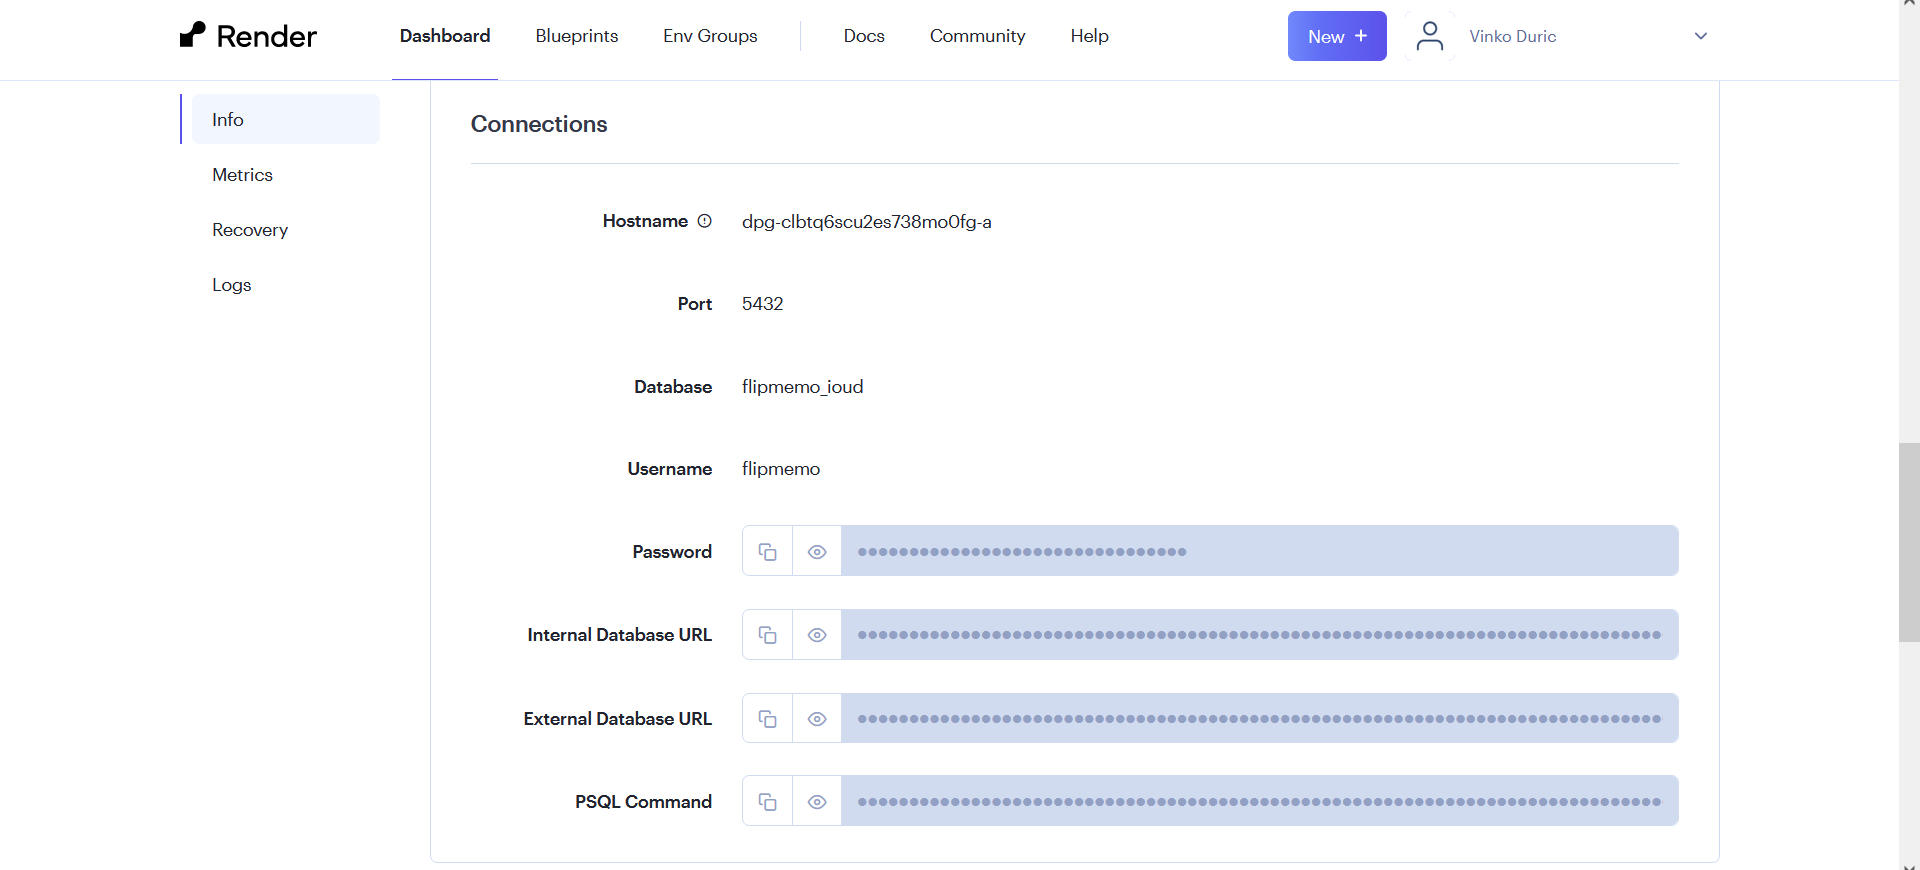
\includegraphics[width=\textwidth]{slike/deploy4.PNG}
				\caption{Render - bitni podaci stvorene baze podataka}
				\label{fig:deployment4}
			\end{figure}
			
			Uz bazu podataka, za puštanje u pogon potrebno je stvoriti novi web servis. Novi web servis stvara se tako što se s početne stranice odabere "New" te zatim "Web Service", slično kao i za bazu podataka. Naša aplikacija se nalazi na GitHub repozitoriju pa je stoga potrebno odabrati prvu opciju od dvije ponuđene na slici 5.6.
			
			\begin{figure}[H]
				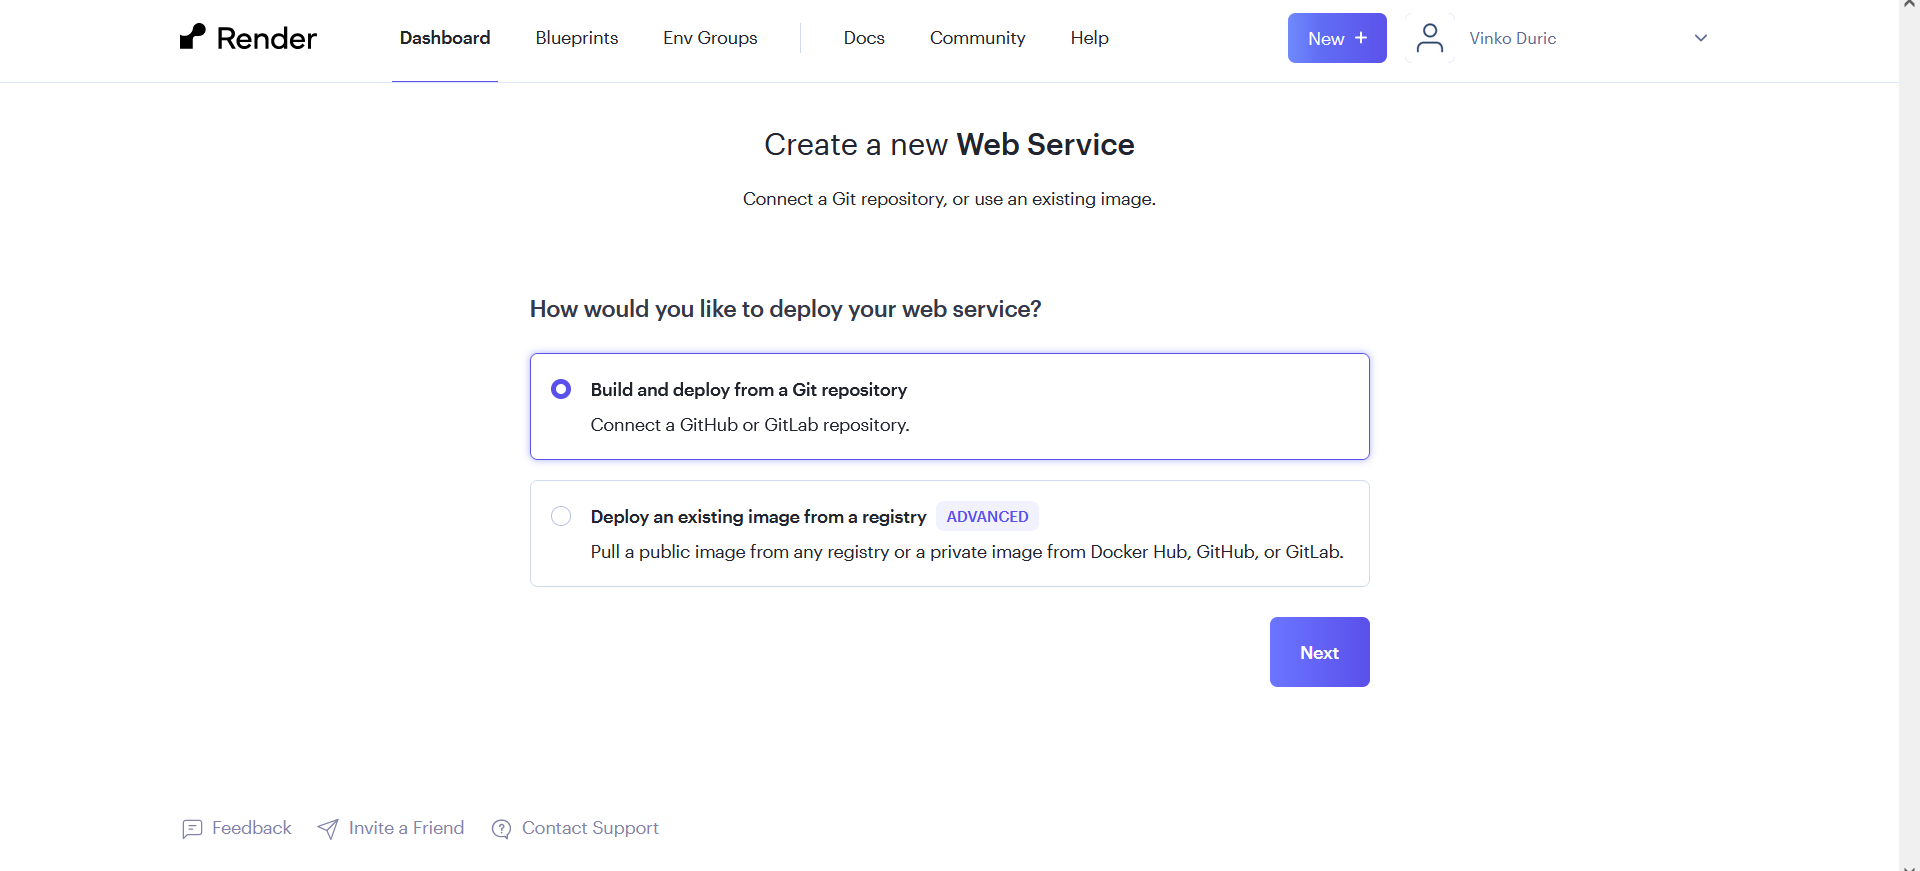
\includegraphics[width=\textwidth]{slike/deploy10.PNG}
				\caption{Render - stvaranje novog web servisa}
				\label{fig:deployment10}
			\end{figure}
			
			Nakon toga potrebno je odabrati željeni repozitorij s kojeg će se izvršiti puštanje u pogon kako je prikazano na slici 5.7.
			
			\begin{figure}[H]
				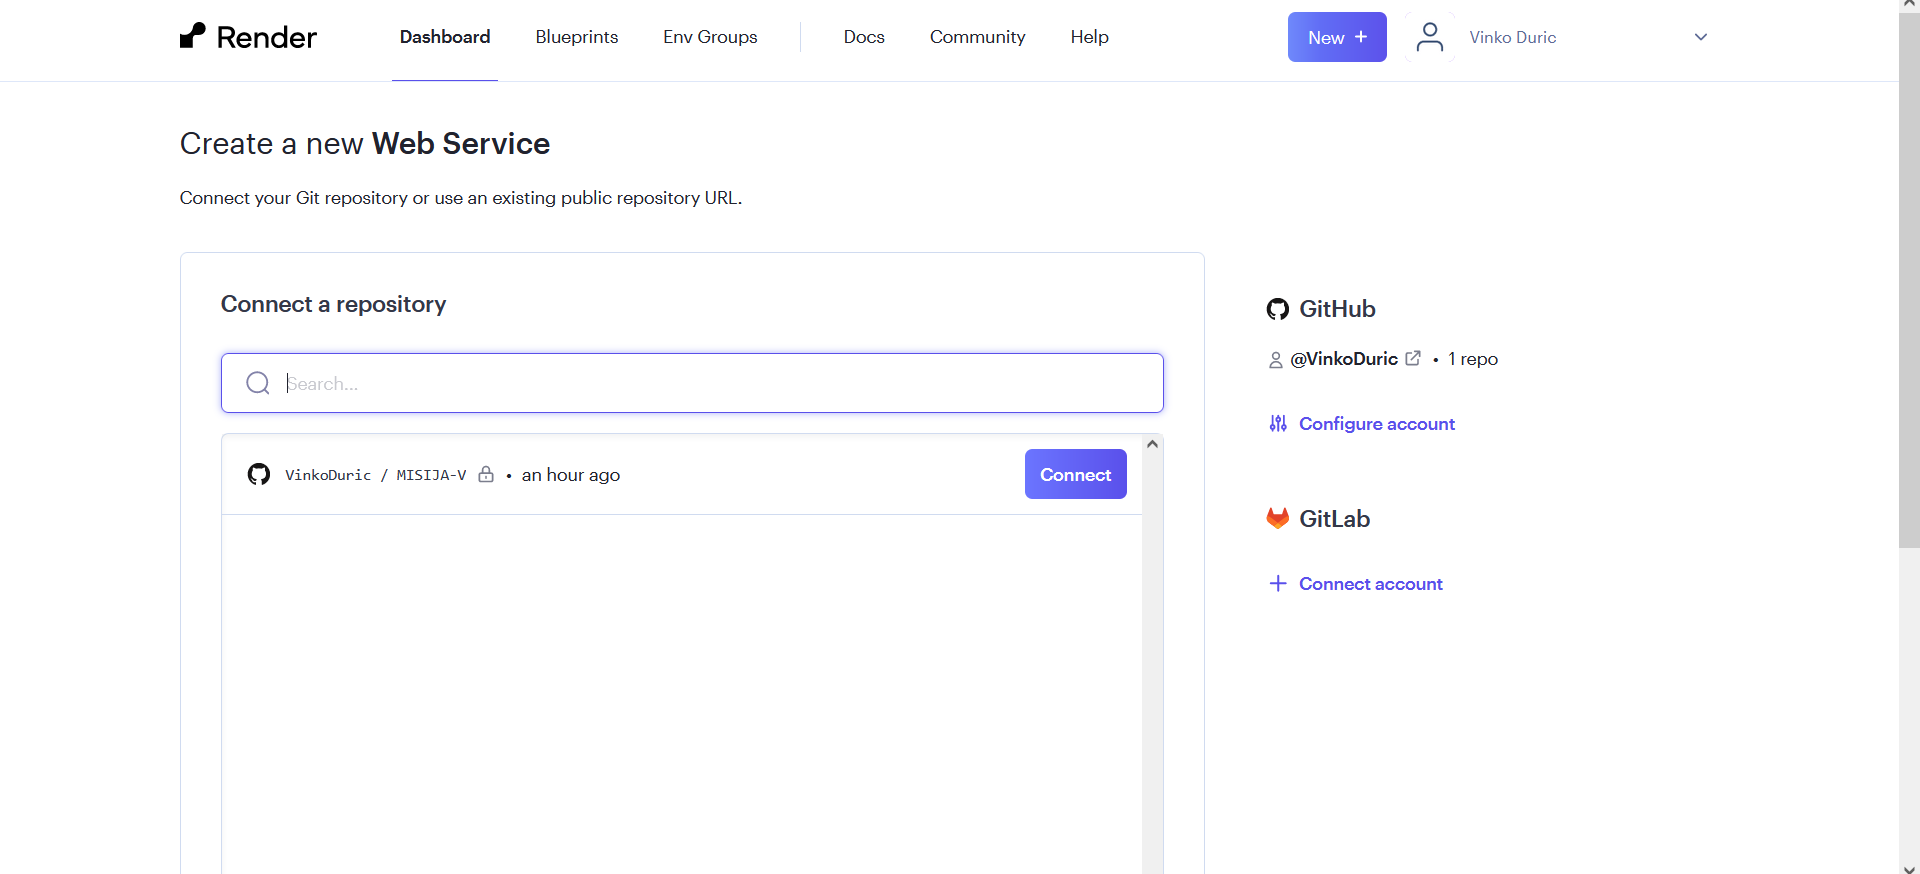
\includegraphics[width=\textwidth]{slike/deploy11.PNG}
				\caption{Render - povezivanje repozitorija}
				\label{fig:deployment11}
			\end{figure}
			
			Za uspješno puštanje u pogon potrebno je podesiti i varijable okruženja. One se podešavaju odabirom opcije "Environment" na lijevoj strani stranice web servisa što je prikazano na slici 5.8.
			
			\begin{figure}[H]
				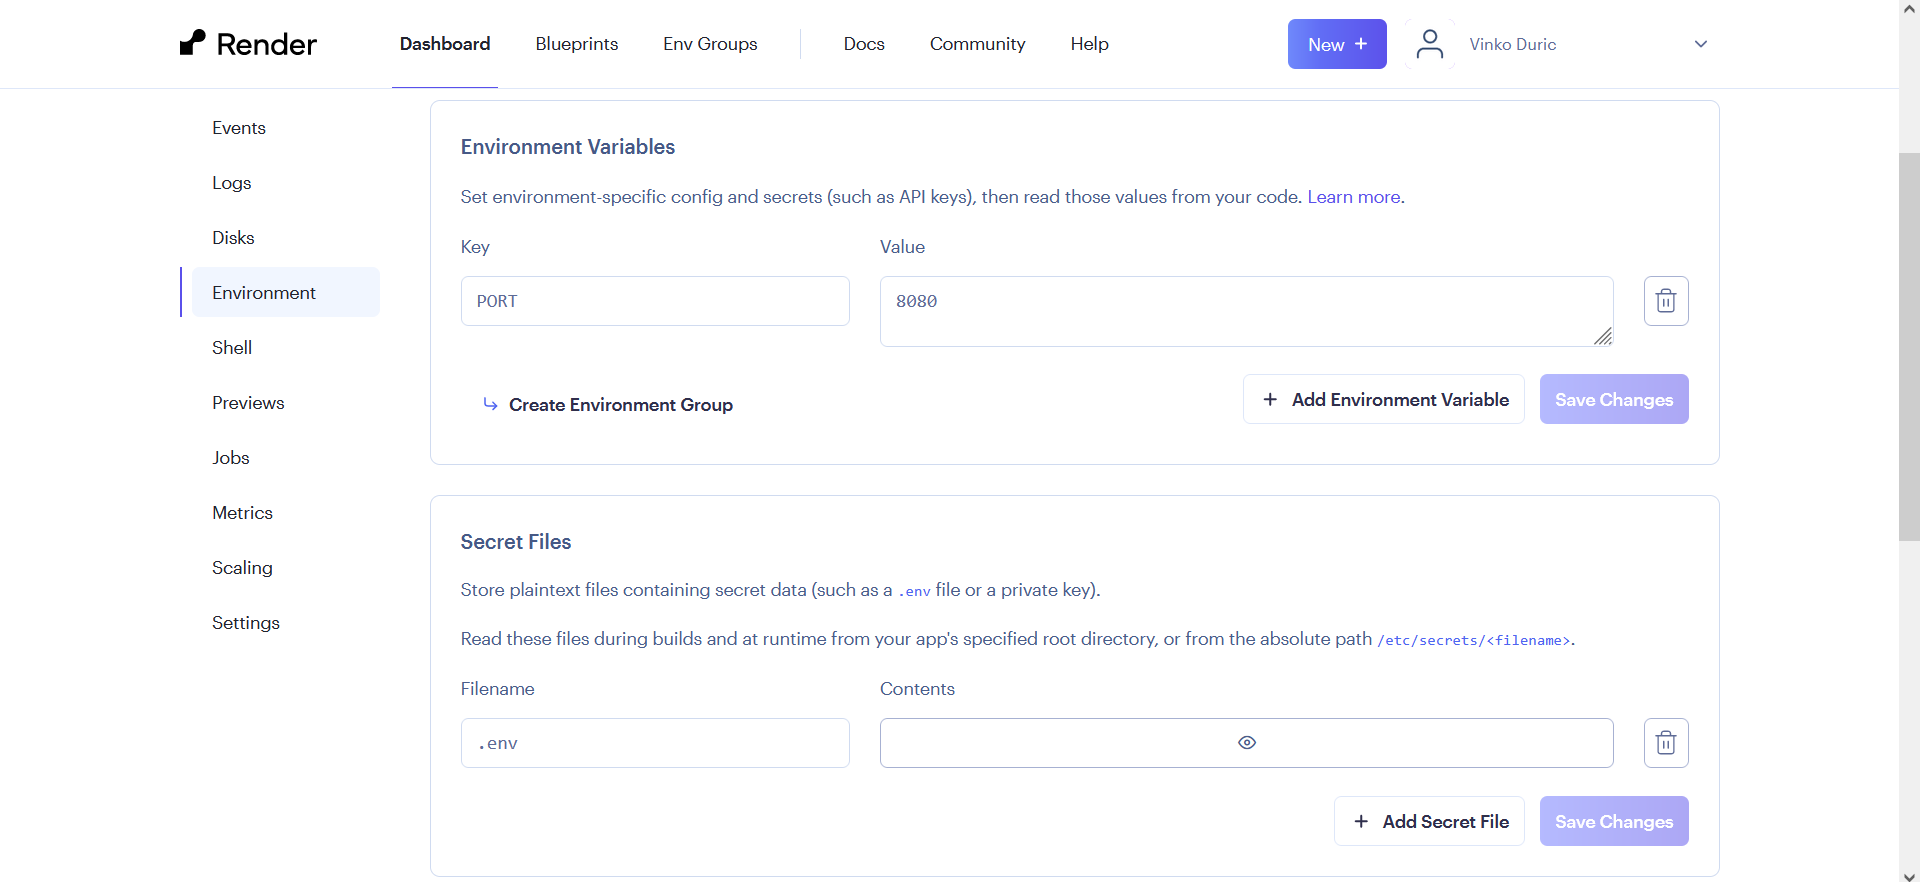
\includegraphics[width=\textwidth]{slike/deploy5.PNG}
				\caption{Render - podešavanje varijabli okruženja}
				\label{fig:deployment5}
			\end{figure}
			
			Primjer ispunjenih varijabli okruženja prikazan je na slici 5.9. Posljednja tri retka ove datoteke ispunjavaju se na temelju podataka iz kreirane baze podataka prikazanih na slici 5.5.
			
			\begin{figure}[H]
				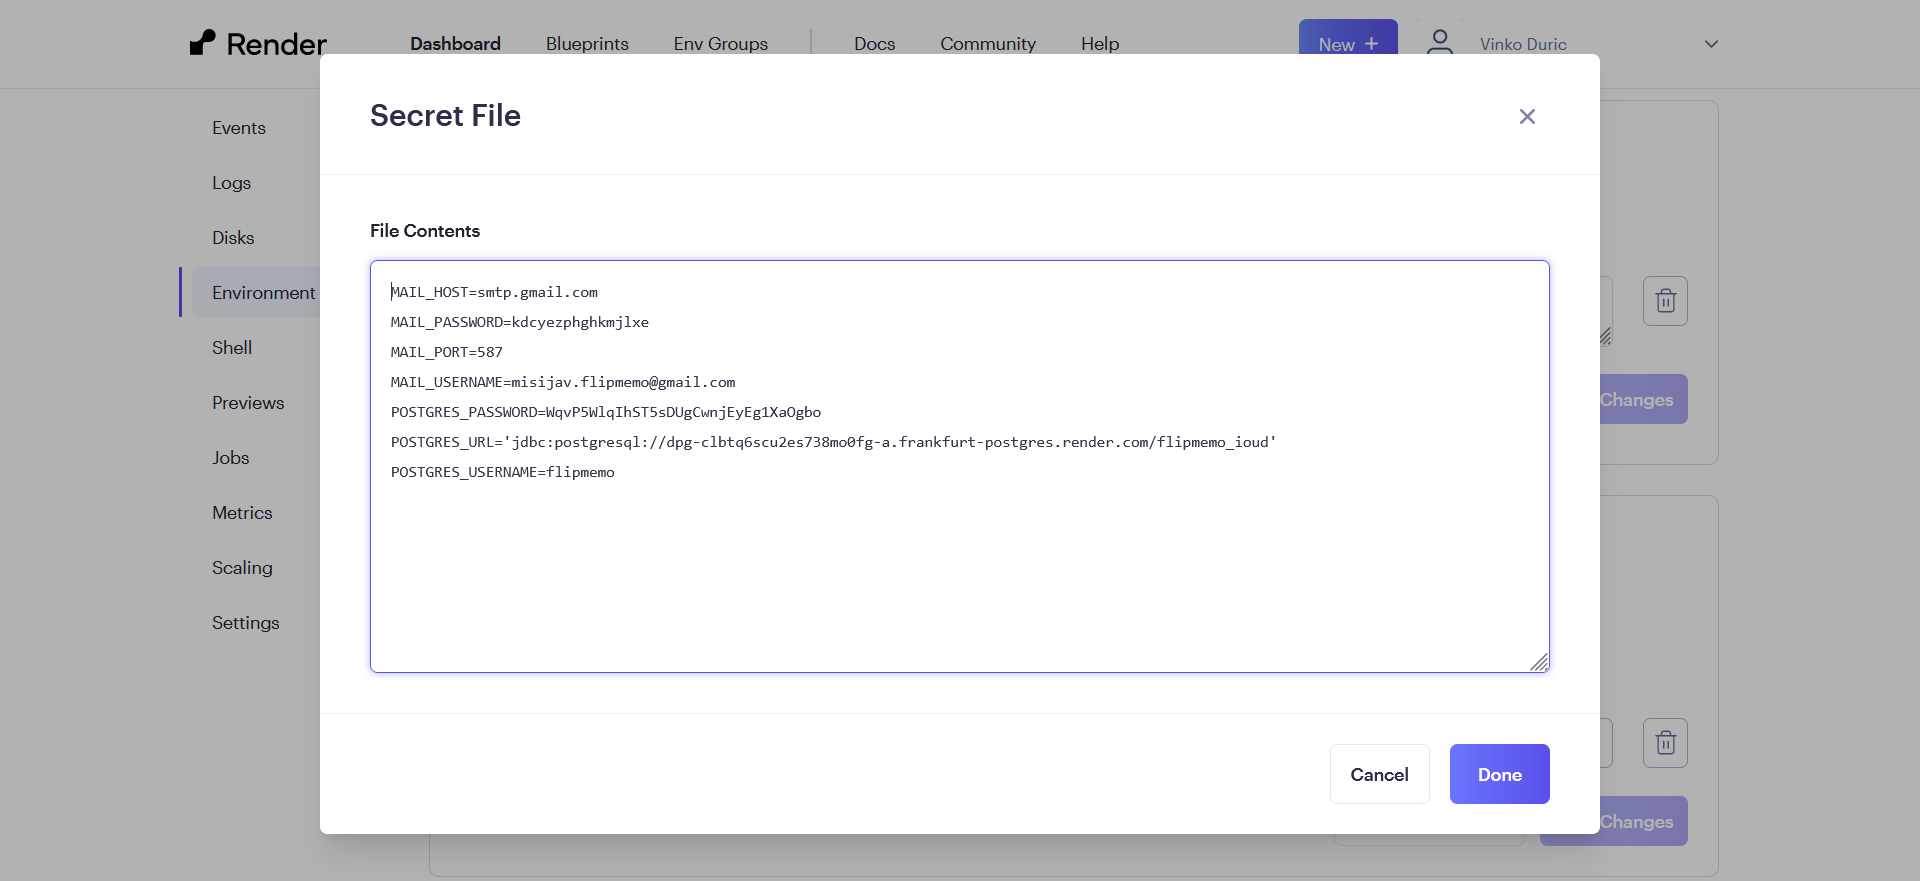
\includegraphics[width=\textwidth]{slike/deploy6.PNG}
				\caption{Render - primjer Secret File datoteke}
				\label{fig:deployment6}
			\end{figure}
			
			U sljedećem koraku potrebno je pokrenuti puštanje u pogon. To radimo na stranici web servisa odabirom opcije "Manual Deploy" te zatim odabirom "Deploy latest commit" iz padajućeg izbornika kako je prikazano slikom 5.10.
			
			\begin{figure}[H]
				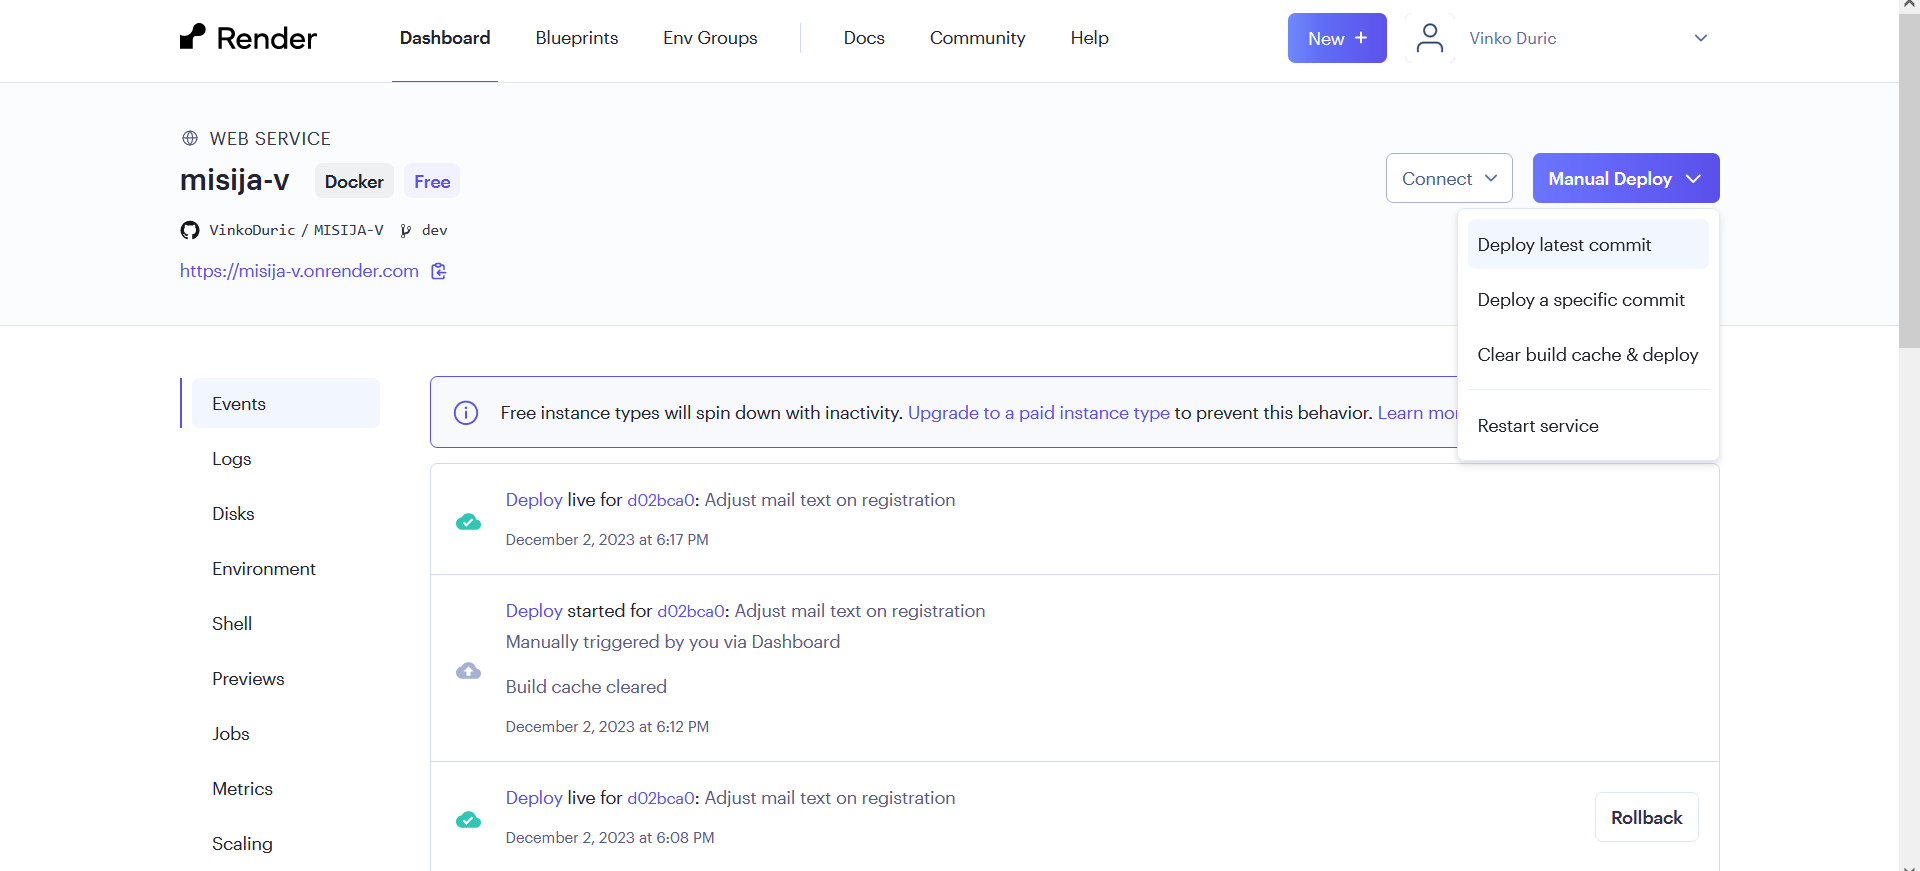
\includegraphics[width=\textwidth]{slike/deploy7.PNG}
				\caption{Render - pokretanje puštanja u pogon}
				\label{fig:deployment7}
			\end{figure}
			
			Slika 5.11 prikazuje primjer poruka koje se ispisuju tijekom procesa puštanja u pogon.
			
			\begin{figure}[H]
				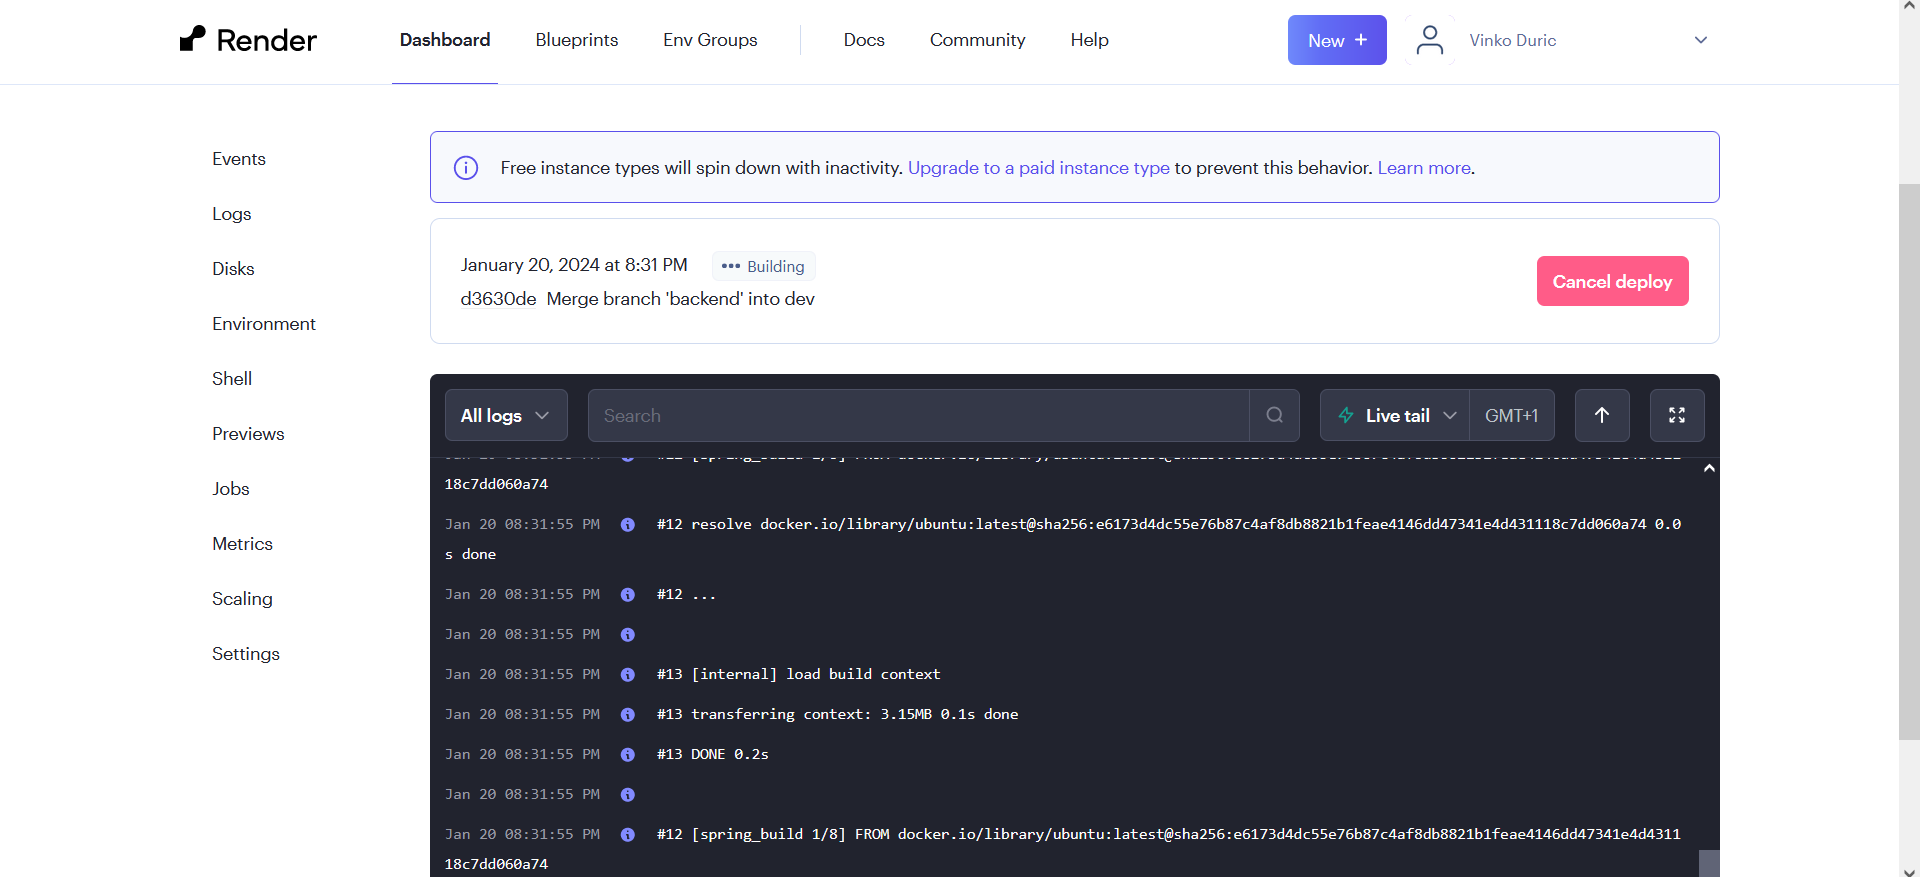
\includegraphics[width=\textwidth]{slike/deploy8.PNG}
				\caption{Render - tijek puštanja u pogon}
				\label{fig:deployment8}
			\end{figure}
			
			Konačno, uspješnost puštanja u pogon možemo vidjeti zadnjom porukom kao što je prikazano na slici 5.12. Ovdje se prikazuju neke poruke poput pokušaja registracije novog korisnika i slično.
			
			\begin{figure}[H]
				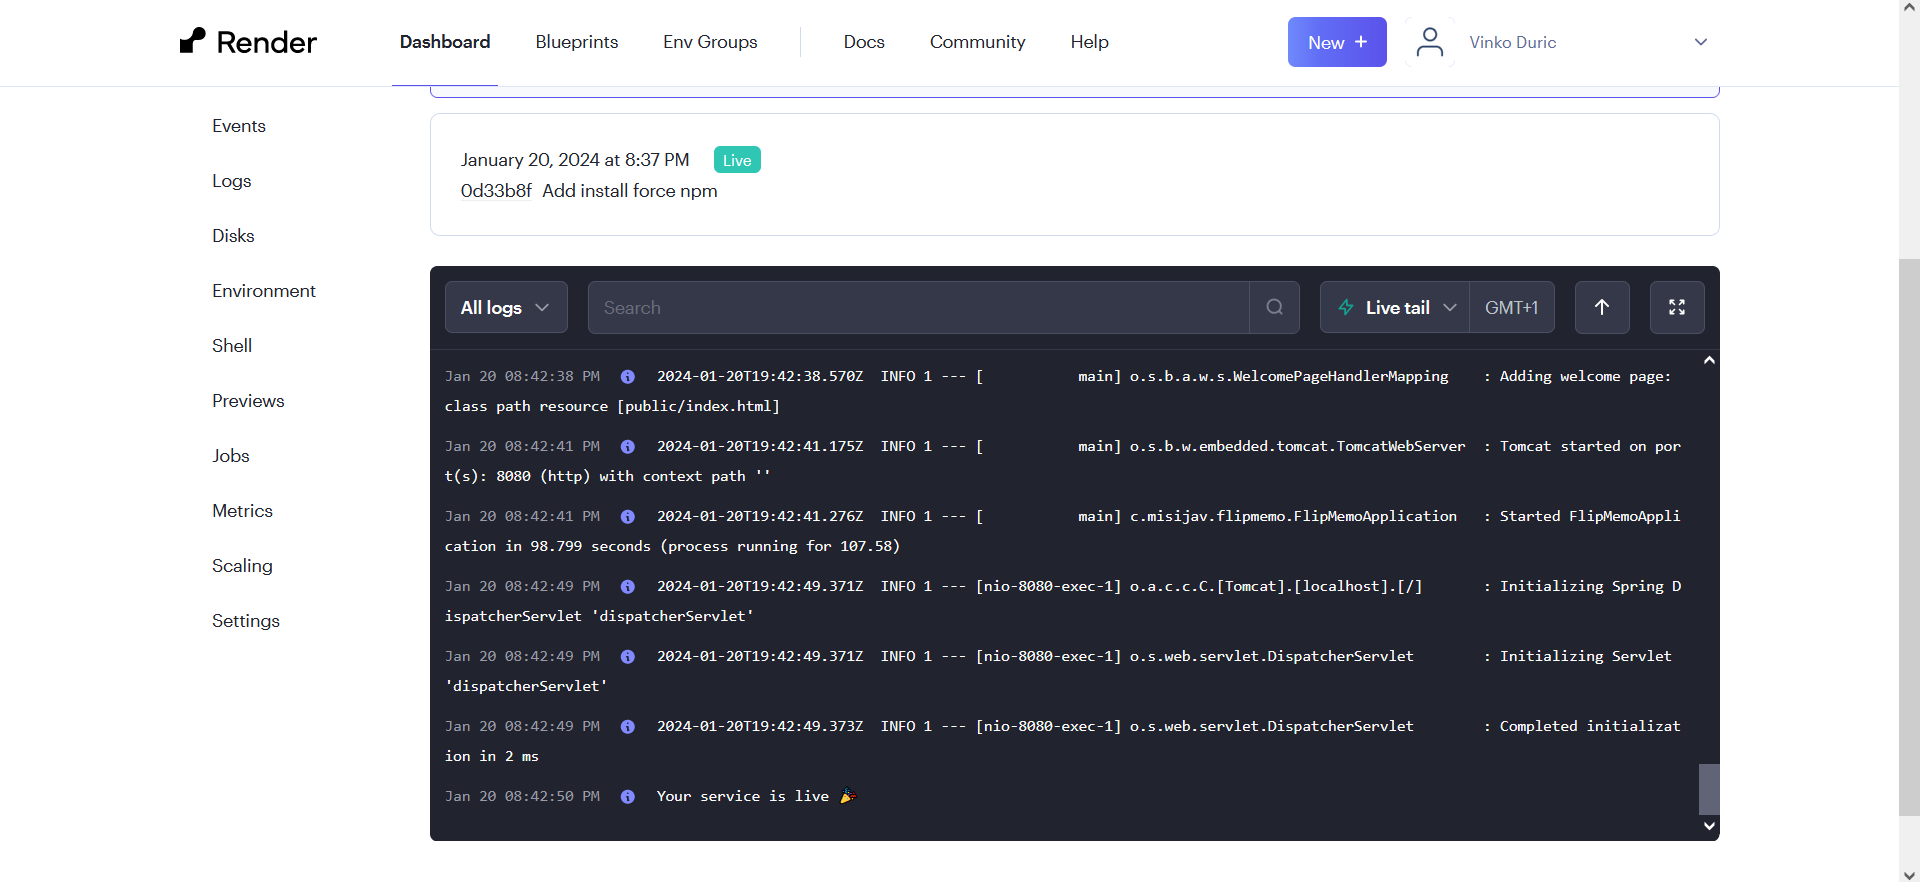
\includegraphics[width=\textwidth]{slike/deploy9.PNG}
				\caption{Render - prikaz poruke o uspješnom puštanju u pogon}
				\label{fig:deployment9}
			\end{figure}
			
			
			\eject 